\chapter{Architecture \& Concepts}

\begin{figure}[ht]
    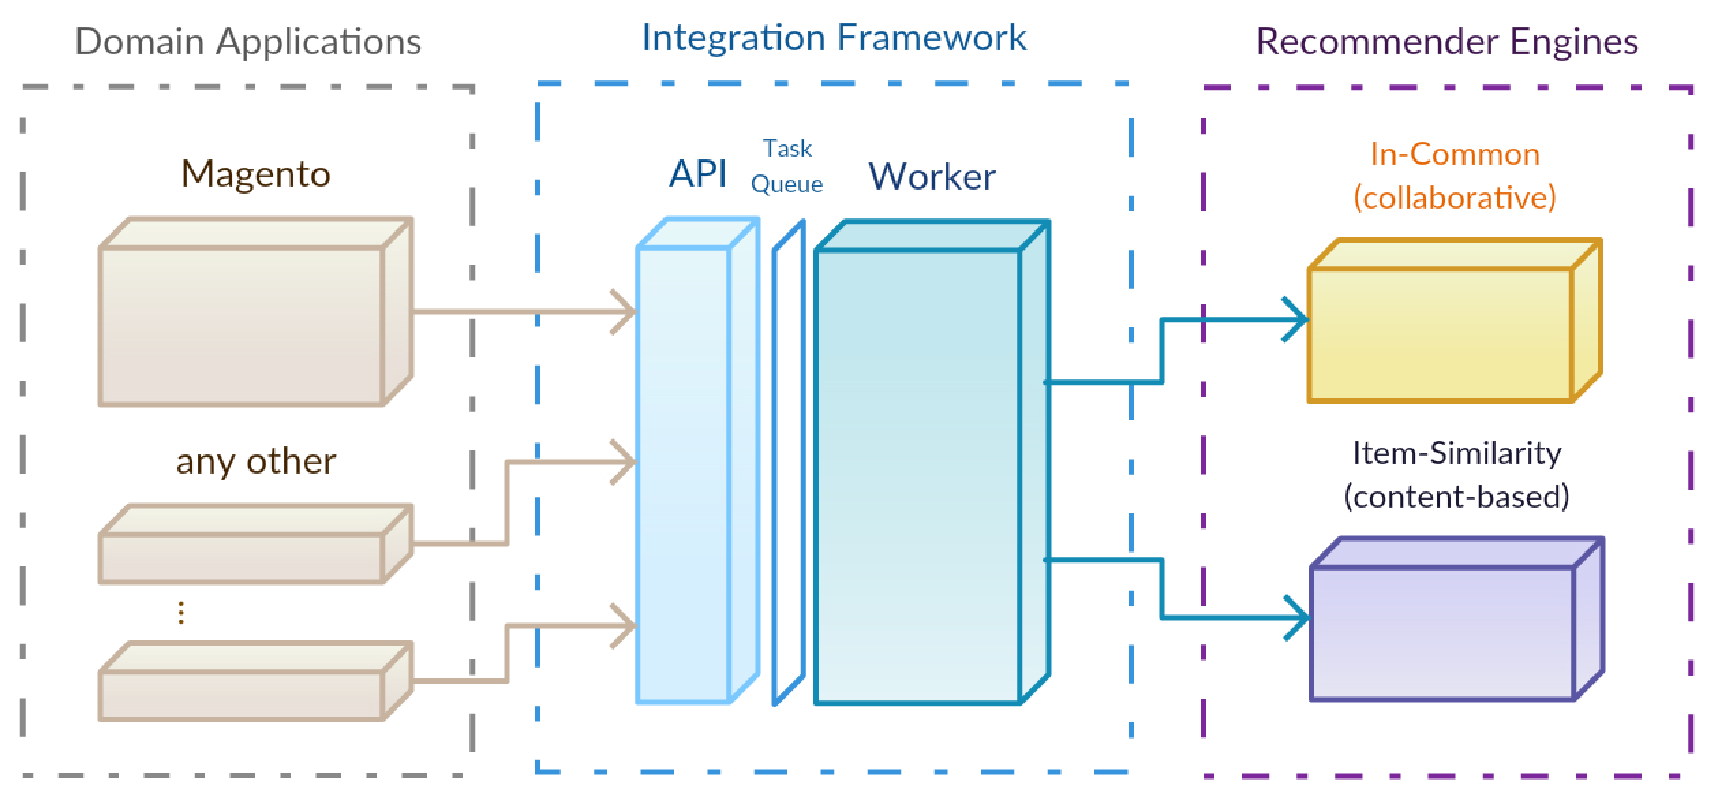
\includegraphics[width=\textwidth,center]{architecture/overview.pdf}
    \caption{Architectural Overview}
    \label{fig:architecture}
\end{figure}

This chapter explains the architecture and core concepts of the solution. Figure \ref{fig:architecture} provides an architectural overview. Although domain and recommender engines have an essential part of this project, the actual targeted solution is the framework. For that reason, this chapter first sets the boundaries of domain and recommender engines and, finally, discusses the framework.

\section{Domain Systems}
\label{architecture-domain-systems}

Throughout this report, \emph{domain systems} refer to existing systems primarily developed for a specific organisation or application, secondarily planning to make use of recommendations and integrate recommendation engines. The definition highlights the fact that these systems are usually built on extensive domain knowledge. Efforts to use recommendations either require domain savvy engineers to gain a recommendation background or recommendation savvy engineers to grasp the domain knowledge. The technology stack -- the collection of all technologies used within a system -- is mostly tailored to the requirements of those systems and may not be the first choice for recommendation requirements. A solution is therefore to develop these requirements as a separate system, which is then integrated into the domain system. As explained in the introduction, this project was about developing an integration framework to support this. Figure \ref{fig:architecture} illustrates that this project supports the integration of as many domain systems as required in a single set-up.

Regarding knowledge, the proposed solution abstracts the internals of both domain and recommender engines. In order for the domain system to provide the requirements for the integration, knowledge about the internals of recommender engines is not required. In fact, to achieve interoperability -- as discussed in section \ref{intro-objectives-abstraction} -- recommender-specific approaches are not wished. For this reason, the emphasis of the integration on the domain systems side lies in the extraction of the data of interest for recommendations. Furthermore the terminology in this data can remain the same as used in the domain systems.

As far as the domain systems are concerned, keeping the integration effort and impact as minimal as possible was of much importance in this project. A typical negative impact of integrating systems is on performance; hence, the integration has been designed to minimise blocking on the domain systems. As a matter of fact, the number of required components, which will be discussed in the next section, has been decreased from proposed three -- \emph{Events}, \emph{Master Data} and \emph{Recommendation} -- to two with \emph{Master Data} being incorporated into \emph{Events}.

\section{Recommender Systems}
\label{architecture-recommender-systems}

As was mentioned in the previous section, the technology stack of domain systems may not be the best fit for recommendation requirements and that a framework was developed to separate them. Originally, it was proposed to implement recommender engines against a uniform database within this framework. Yet while working on the project, it became obvious that the same technological fitness concern applied to the framework as well; in the sense that the technology stack of the framework may not be the best suited for recommender engines. Furthermore, the best suitable technology stack may differ substantially among recommender engines themselves.

Therefore it was decided to design recommenders as individual systems which allows the utilisation of not only the most suitable technology stack such as database management systems and programming languages but also existing, third-party recommender engines e.g. \emph{LensKit} or \emph{Apache Mahout}.

\section{Framework}
\label{architecture-framework}

\begin{figure}[ht]
    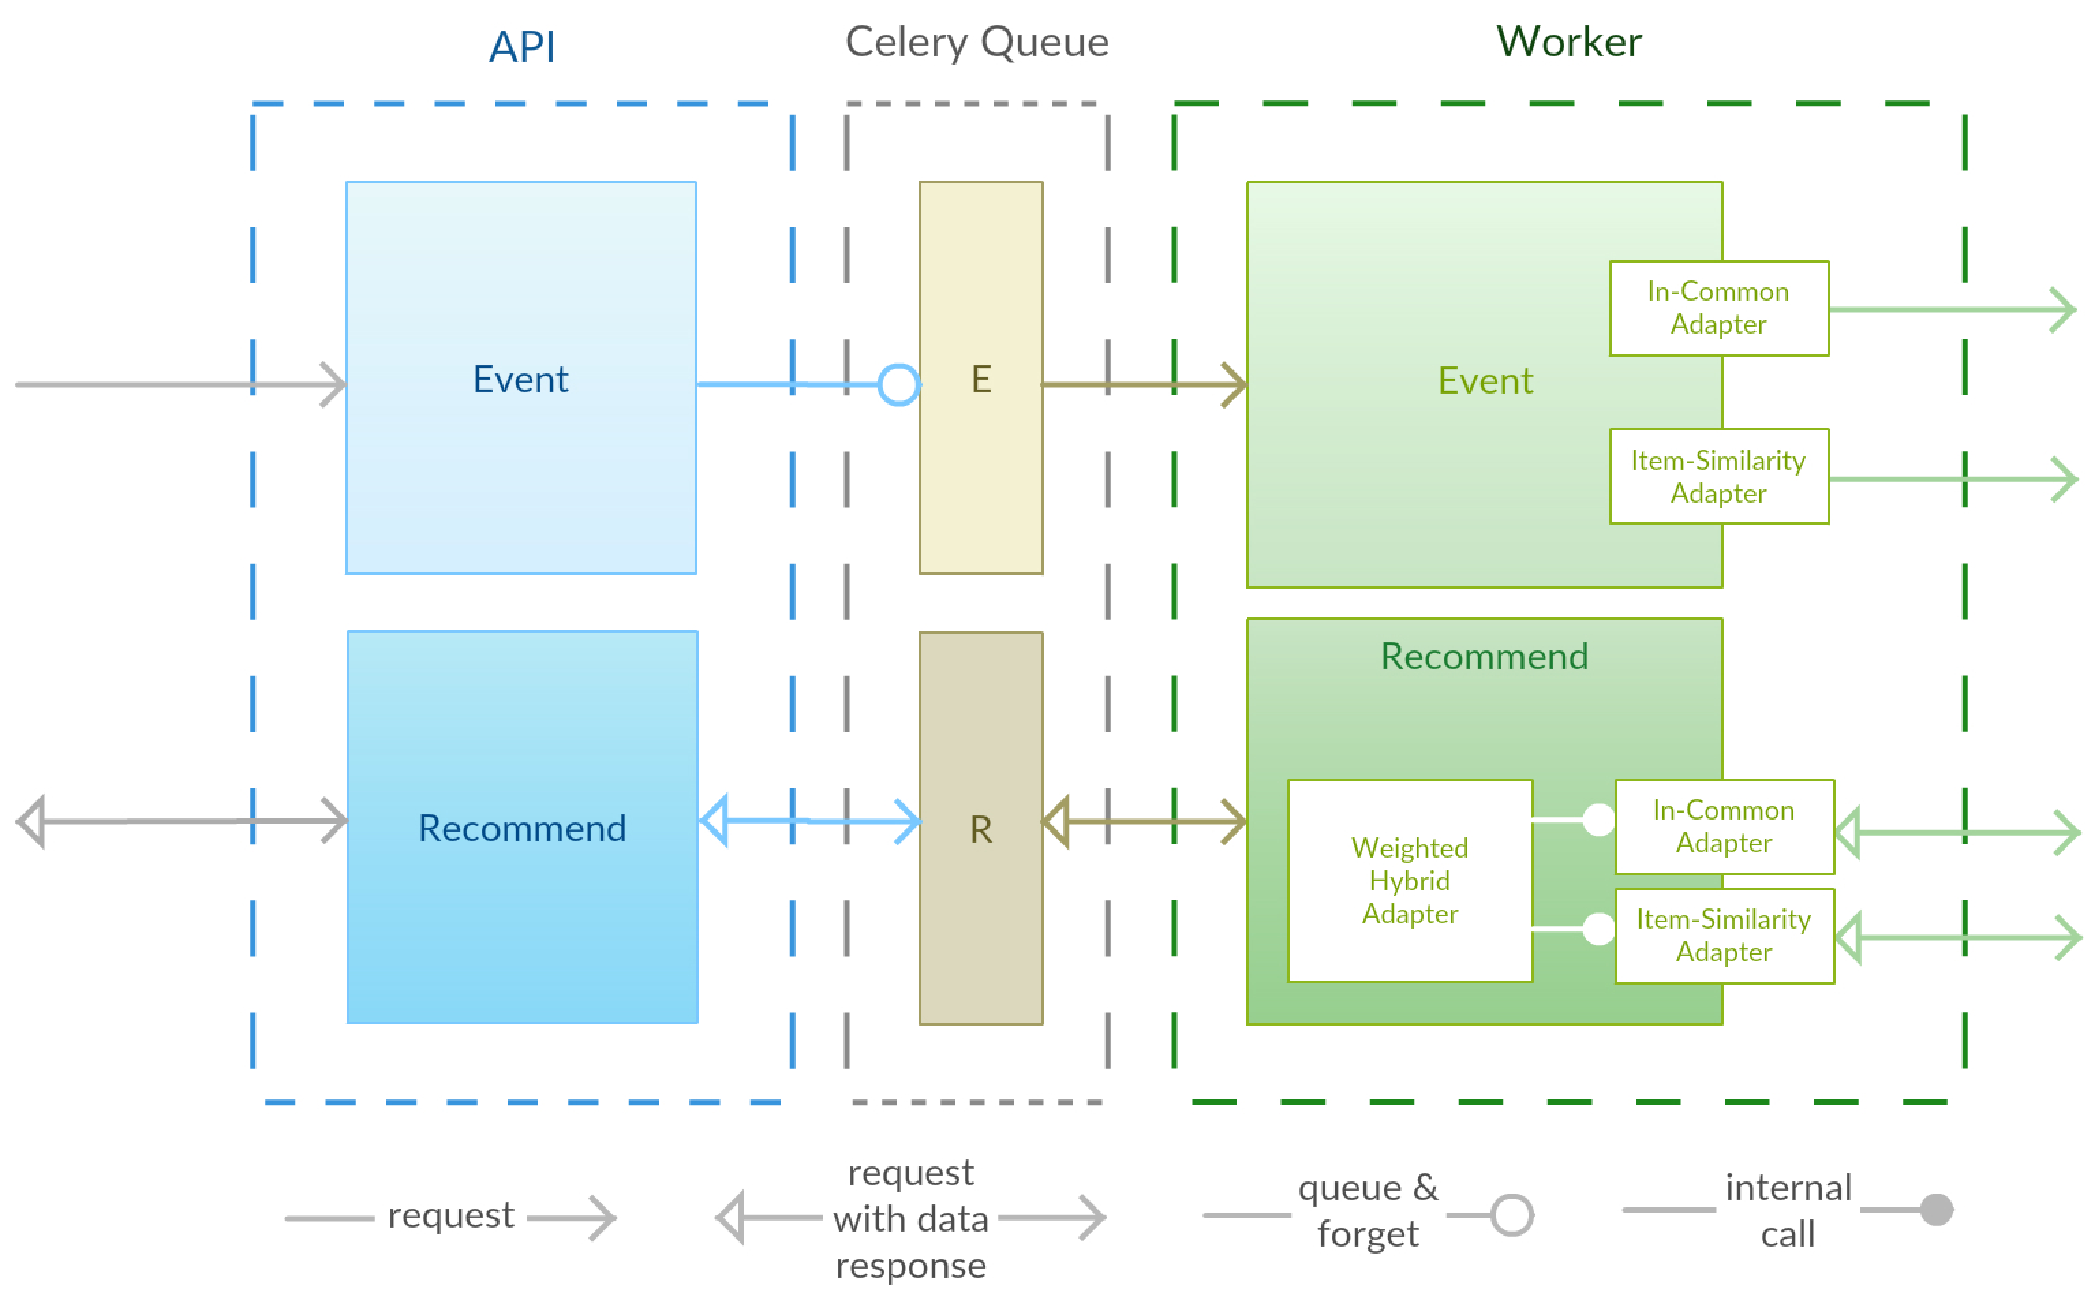
\includegraphics[width=\textwidth,center]{architecture/framework.pdf}
    \caption{Framework Design}
    \label{fig:architecture-framework}
\end{figure}

In the present report, the framework relates to the centre piece of this project while the domain systems and recommender engines primarily serve to demonstrate its capabilities. Above all, the framework is an integration tool to glue domain systems and recommendation engines in a way which allows interoperability, abstraction as well as easy integration, and is technologically unbiased -- those being the ultimate objectives of this project as outlined in section \ref{intro-objectives}. In that sense, it can be also seen as a middleware.

Figure \ref{fig:architecture-framework} shows a more detailed diagram of the framework and makes two characteristics immediately visible:

First, \emph{Event} and \emph{Recommend} are distinguished throughout the design of the framework. This reflects the \emph{service-oriented architecture (SOA)} as discussed in the project proposal. SOA suggests expressing features as services and comes with principles such as \emph{loose coupling}, \emph{abstraction} and \emph{reusability} -- matching the objectives of the project which were already outlined in detail.

Second, the framework is horizontally separated into layers which reflects the proposed \emph{multi-layered architecture}. However, the project proposal suggested four layers which differ from the final solution: \emph{interface}, \emph{configuration}, \emph{recommendation} and \emph{persistence}. The API covers the interface layer whereas the configuration layer is more or less the workers. The layers recommendation and persistence are now regarded by the individual recommender engines.

\subsection{Concepts}

This section describes concepts and terminology used in the framework. Those are also referred to throughout the report.

\subsubsection{Engine}

An \emph{engine} basically refers to a recommender engine to be used in the framework. An engine is primarily described by the algorithmic approach rather than its practical use case. As an illustration, the \emph{In-Common} engine -- implemented as part of this project -- finds \emph{items other users who have experienced the same items as the current user have experienced but the current user has not yet}. One of the use cases in practice is based on customers viewing products, so a concrete case of the previous.

\subsubsection{Engine Adapter}

An \emph{engine adapter} is a piece of software code in the framework, which does the interaction with an engine. Every engine requires an engine adapter and thus the part of the framework which knows how the respective recommendation engine works.

The only formal requirement of engine adapters is that they implement handlers for events the recommender has subscribed to. The nature of the interaction between engine adapter and engine mainly depend on the technical architecture of the engine. It can happen that the engine does not provide an interface for the engine adapter to hook into -- especially with engines, which were not originally designed to work with this framework. In this case, it may be required to implement a counter piece on the engine technology.

This project only demonstrates engine adapters with RESTful interfaces.

\subsubsection{Events}

An \emph{event} relates to anything recommenders need to be notified about. For collaborative recommenders these are usually user behaviour such as \emph{customer viewed product} or \emph{user favourited movie}.

Content-based recommenders on the other hand would usually like to be notified about data changes such as items added, updated or removed. Events have an alphanumeric subject as well as a payload. Originally, it was proposed to have a separate \emph{master data} concept as well. It was dropped in favour of incorporating it into the event concept due to the fact that even master data changes are triggered by some kind of event such as creation and removal.

\subsubsection{Recommender}

A \emph{recommender} is an instance or in other words use case of a recommender engine. In example, \emph{common_products_viewed} and \emph{common_products_wishlisted} are recommenders utilising the \emph{In-Common} engine. Recommenders subscribe to events such as \emph{viewed_product}. Additionally, they define a taxonomy -- which is explained in a bit. Figure \ref{fig:architecture-framework-recommender} shows a recommender configuration used in the project.

\begin{figure}[ht]
    \begin{minted}{xml}
    <recommenders>
        <recommender name="common_products_wishlisted" engine="in_common">
            <on event="added_to_wishlist" do="post" />
            <on event="removed_from_wishlist" do="delete" />
            <taxonomy inherit="user_product">
                <taxon name="relationship">WISHLISTED</taxon>
            </taxonomy>
        </recommender>
    </recommenders>
    \end{minted}
    \caption{Recommender Configuration Example}
    \label{fig:architecture-framework-recommender}
\end{figure}

\subsubsection{Hybrids}

A \emph{hybrid recommender} is a composite of two or more recommenders -- in this case components. Hybrid recommenders do not subscribe to events nor define a taxonomy. However they still specify an engine but of type \emph{hybrid engine} which only provides a call back to be called when a recommendation query is received. This call back can utilise its components and return a list of recommendations. As visible in Figure \ref{fig:architecture-framework}, these hybrid engines are implemented within the framework.

This project implemented a \emph{weighted} hybrid recommender, which queries all recommenders and combines their recommendations using a linear formula. A potential \emph{switching} hybrid recommender would choose one of the components based on some criterion. Thus it is deliberately vague as there are a variety of hybrid recommendation approaches. Figure \ref{fig:architecture-framework-hybrid-recommender} illustrates an example hybrid recommender configuration.

\begin{figure}[ht]
    \begin{minted}{xml}
        <hybrid_recommender name="interesting_products" engine="weighted">
            <components>
                <component name="views" recommender="common_products_viewed" />
                <component name="wishlists" recommender="common_products_wishlisted" />
            </components>
        </hybrid_recommender>
    \end{minted}
    \caption{Hybrid Recommender Configuration Example}
    \label{fig:architecture-framework-hybrid-recommender}
\end{figure}

\subsubsection{Taxonomy}

A \emph{taxonomy} is a mapping concept between domain and recommender terminologies as those are unknown to each other. It consists of \emph{taxons} which define a map for a single term. It can also inherit from another taxonomy. Before passing a payload to a recommender engine, it is going through the mapping process first. Given the taxonomy definition in Figure \ref{fig:architecture-framework-taxonomy}, a payload of \texttt{user=halil, user_id=2, limit=10} would become \texttt{subject=halil, subject_id=2, limit=10, relationship=VIEWED}.

\begin{figure}[ht]
    \begin{minted}{xml}
        <taxonomies>
            <taxonomy name="base">
                <taxon name="limit">limit</taxon>
            </taxonomy>
            <taxonomy name="user" inherit="base">
                <taxon name="subject">user</taxon>
                <taxon name="subject_id">user_id</taxon>
                <taxon name="relationship">VIEWED</taxon>
            </taxonomy>
        </taxonomies>
    \end{minted}
    \caption{Taxonomy Configuration Example}
    \label{fig:architecture-framework-taxonomy}
\end{figure}

\subsection{API}

The \emph{application programming interface (API)} is the endpoint (\emph{server}) for domain systems (\emph{client}) to interact with the framework. It is the only subsystem of the framework, which is exposed to other systems depending on the network configuration. The API adopts the architectural style \emph{representational state transfer (REST)} -- and is thus \emph{RESTful} -- via the \emph{hypertext transfer protocol (HTTP)} which is one of the fundamental protocols of the \emph{Internet} and \emph{world wide web}. Resources and actions define REST APIs. Resources are uniquely referenced with \emph{uniform resource locators (URLs)}. Actions specify the operation to happen on a resource. Latter is described by REST as \emph{HTTP vocabularies} amongst others \emph{GET}, \emph{POST} and \emph{DELETE}. Both URLs and HTTP vocabularies are basics of the Internet and are almost self-explanatory which results in more compact documentation \cite{fielding00}.

An essential property of REST is \emph{statelessness} and says that the server should not remember any state of the client. \citet{fielding00} further states that statelessness improves \emph{visibility}, \emph{reliability} and \emph{scalability}. Visibility is improved by the fact that a  request by a client has all information necessary to understand. Reliability is improved because a request is not affecting others and makes recovery of partial failures easier. Finally, better scalability can be observed as the server does not need to manage state data between requests.

The framework has two APIs: Event handles event notifications as \emph{POST} requests whereas Recommend handles recommendation queries as \emph{GET} requests. As far as the framework is concerned, its API bears no business logic at all and hands requests over to the workers via a task queue which is going to be covered in the next section.

\subsection{Task Queue}

A \emph{task queue} is a software system for managing tasks via \emph{message queue} systems. The latter store messages sent by a publisher into a queue and enable one or more consumers to read messages from the queue. Amongst other benefits, message queues allow communication between independent systems and can help scaling by distributing messages to more than one consumer. Similarly, task queue systems offer a mechanism to run tasks on independent systems and distribute them to a group of processes. It hides the internals such serialisation of task contexts into messages as well as handling errors and responses.

Figure \ref{fig:architecture-framework} illustrates the task queue system \emph{Celery} and the following queues used: \emph{Event} and \emph{Recommend}. Albeit task queue systems can manage different tasks via a single queue, it was decided to use designated queues to give prioritisation of recommendations over event tasks. Practically, it means that a recommendation query of a customer has to be processed sooner than eventual events which can be a lot. The Event API runs tasks asynchronously and does not wait for a result (\emph{queue \& forget}) whereas the Recommend API waits for the result -- namely a list of recommended items.

\subsection{Workers}

The \emph{workers} are background processes called via aforementioned task queues. Whereas the API is only considered a request handler, the workers are doing the actual processing. Similar to API and queues, they are also divided into \emph{Event} and \emph{Recommend} workers.

Workers are designed to scale horizontally by running more instances.
